%!TEX root = ../thesis.tex

%hakon -- macro-level simulation results chapter

\chapter{Macro-Level Simulation Results}
\label{ch:macro_results}

\section{Experimental Setup}
\label{sec:macro_setup}

%hakon
All macro simulations are run using the MATLAB/Simulink implementation of the SIRVHDB model described in Chapter~\ref{ch:macro_model}.
Unless otherwise stated, the following initial conditions are used: $I_c(0) = 0.01$, $S_c(0) = 0.99$, with all other compartments initialised to zero.
The vaccination rates are $\nu_1 = 0.001$ and $\nu_2 = 0.002$ for City~1 and City~2 respectively.
The hospital capacity $H_{{\mathrm{cap}},c}$ is set at a level consistent with the reported Norwegian ratio of approximately 5 beds per 100\,000 inhabitants \citep{kohler2021}.
Compartment values are normalised, representing proportions of the total city population rather than absolute counts.

Two simulation horizons are used: $T = 150$~days for direct comparison with the micro model, and $T = 500$~days for examining long-term wave dynamics and sustained MPC behaviour.

\section{Baseline Epidemic Dynamics (No Control)}
\label{sec:baseline_macro}

%hakon
Figure~\ref{fig:baseline_macro} shows the epidemic dynamics of the macro model without control.
Due to the symmetric initial conditions and similar parameters across both cities, the two cities exhibit nearly identical behaviour.
The infected compartments $I_c$ and $I_{v,c}$ are combined and presented as the total infected population $I_{c,{\mathrm{total}}}$ for clarity.

\begin{figure}[ht]
  \centering
  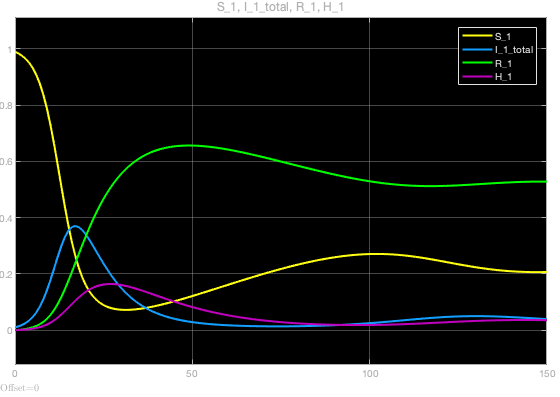
\includegraphics[width=0.75\textwidth]{Figures/hakon/epi_c1_SIRH}
  \caption{%hakon
    Selection of compartments from City~1, simulated over 150~days without control.
    The susceptible population declines as the infected compartment rises to a peak,
    followed by recovery and growth of the hospitalised and immune populations.}
  \label{fig:baseline_macro}
\end{figure}

Without intervention, the infected population rises sharply in the first 30--40 days and reaches a peak before declining as the susceptible pool is depleted.
The healthcare demand follows a similar trend with a delayed peak of approximately 0.32 (normalised), and a slower decline compared to infections.
After reaching a minimum, the infection level begins to slowly increase again due to waning immunity returning previously recovered and vaccinated individuals to the susceptible pool.

\section{City-to-City Interaction}
\label{sec:city_interaction}

%hakon
To isolate the effect of intercity interaction mechanisms, one city is initialised with $S_c(0) = 1$ and all other compartments zero, while the other city starts with $S_c(0) = 0.99$ and $I_c(0) = 0.01$.
Figure~\ref{fig:city_travel} and Figure~\ref{fig:city_commute} show the resulting infection dynamics under travel-only and commuting-only interaction respectively.

\begin{figure}[ht]
  \centering
  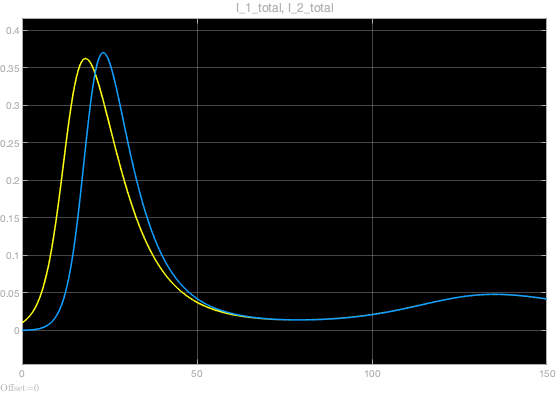
\includegraphics[width=0.75\textwidth]{Figures/hakon/I_total_travel}
  \caption{%hakon
    Infection dynamics in both cities under travel-only interaction (commuting disabled).
    The infection spreads from the seeded city to the initially uninfected city,
    though with a longer delay than in the commuting-only scenario.}
  \label{fig:city_travel}
\end{figure}

\begin{figure}[ht]
  \centering
  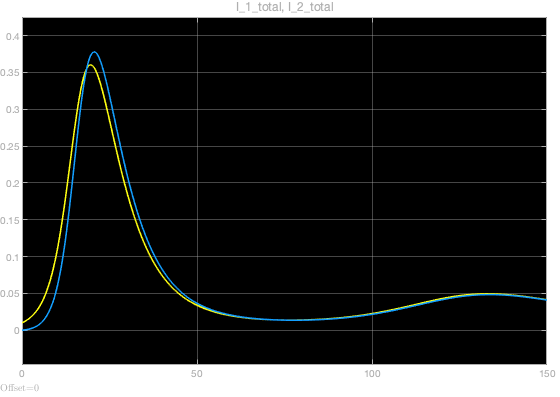
\includegraphics[width=0.75\textwidth]{Figures/hakon/I_total_commute}
  \caption{%hakon
    Infection dynamics in both cities under commuting-only interaction (travel disabled).
    Cross-city spread is faster than in the travel-only case, demonstrating
    the strong coupling introduced by the commuting-based mixing model.}
  \label{fig:city_commute}
\end{figure}

In both scenarios the infection spreads from the initially infected city to the other city.
When commuting is disabled, the spread is more delayed compared to the commuting-only case.
This demonstrates that both interaction mechanisms contribute to intercity transmission, and that the model correctly captures the intended dynamics of epidemic spreading between cities.
The strong coupling produced by the commuting matrix means that the two cities behave almost as a single large population under typical parameter settings, resembling the relationship between two cities in the same greater metropolitan area.

\section{Waning Immunity}
\label{sec:waning}

%hakon
Waning immunity is a critical feature of the model because it prevents the population from reaching permanent immunity and allows for repeated epidemic waves.
Figure~\ref{fig:no_waning} shows the dynamics without waning immunity, and Figure~\ref{fig:with_waning} shows the corresponding dynamics with waning immunity enabled, both over an extended 500-day simulation horizon.

\begin{figure}[ht]
  \centering
  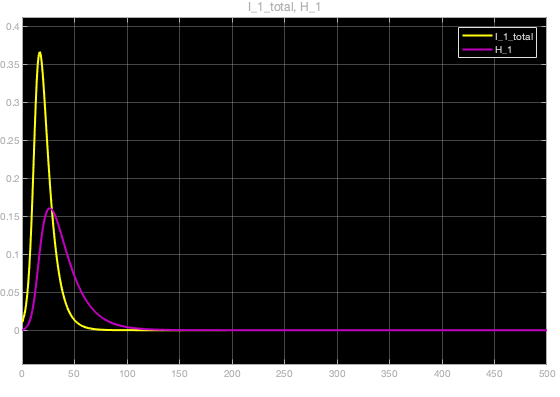
\includegraphics[width=0.75\textwidth]{Figures/hakon/IH_500_noW}
  \caption{%hakon
    Infection and healthcare dynamics over 500~days \emph{without} waning immunity
    ($\omega_R = \omega_V = 0$). The infection dies out after a single wave
    and the healthcare demand approaches zero after approximately 100 days.}
  \label{fig:no_waning}
\end{figure}

\begin{figure}[ht]
  \centering
  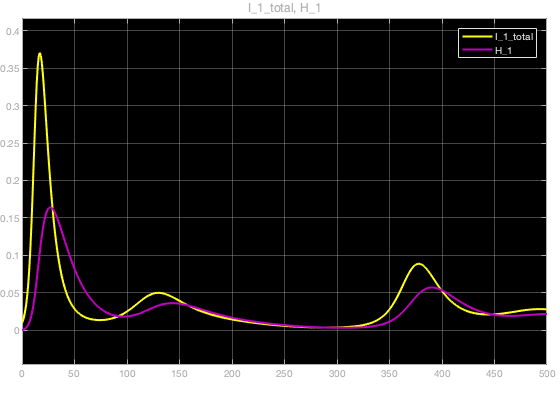
\includegraphics[width=0.75\textwidth]{Figures/hakon/IH_500_waning}
  \caption{%hakon
    Infection and healthcare dynamics over 500~days \emph{with} waning immunity
    ($\omega_R = 1/110$, $\omega_V = 1/140$). Multiple infection waves emerge
    as previously immune individuals return to the susceptible pool.}
  \label{fig:with_waning}
\end{figure}

Without waning immunity, the infections decline to zero after approximately 60~days, and the healthcare demand approaches zero after around 100~days.
When waning immunity is included, multiple waves of infection emerge over time.
This result confirms that waning immunity is essential for the model to exhibit realistic multi-wave epidemic dynamics consistent with the observed behaviour of COVID-19.

\section{Macro Model with MPC}
\label{sec:macro_mpc_results}

%hakon
This section presents simulation results from the macro model under MPC feedback.
The purpose is to evaluate both the performance of the MPC controller and the behaviour of the epidemic system under different conditions.

\subsection{Baseline Comparison (150~Days)}
\label{sec:mpc_150}

%hakon
Figure~\ref{fig:mpc_no_150} shows the development of total infections and healthcare demand across both cities without intervention over 150~days.
Figure~\ref{fig:mpc_yes_150} shows the corresponding trajectories when the MPC is active.

\begin{figure}[ht]
  \centering
  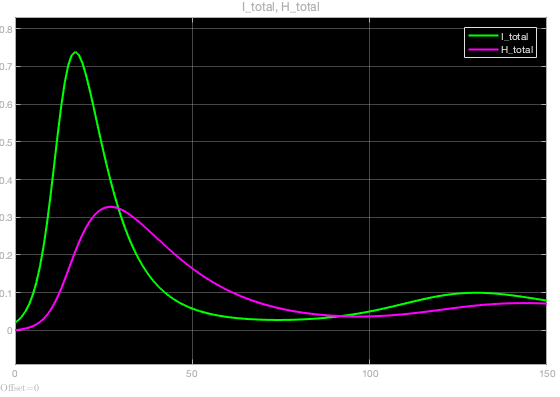
\includegraphics[width=0.75\textwidth]{Figures/hakon/B_150_no}
  \caption{%hakon
    Total infections and healthcare demand across both cities without MPC intervention
    over 150~days. The infection peak reaches approximately 0.73 (normalised);
    the healthcare demand peak reaches approximately 0.32.}
  \label{fig:mpc_no_150}
\end{figure}

\begin{figure}[ht]
  \centering
  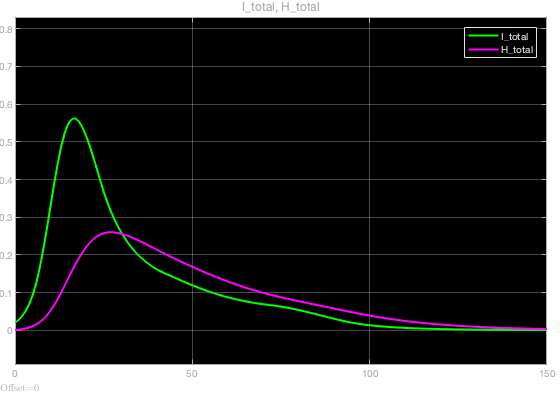
\includegraphics[width=0.75\textwidth]{Figures/hakon/B_150_mpc}
  \caption{%hakon
    Total infections and healthcare demand across both cities with MPC intervention
    over 150~days. The infection peak is reduced to approximately 0.56;
    the healthcare demand peak falls to approximately 0.26.}
  \label{fig:mpc_yes_150}
\end{figure}

Under MPC control, the infection peak is reduced from approximately 0.73 to 0.56 (a 23\% reduction), while the healthcare demand peak falls from 0.32 to 0.26 (a 19\% reduction).
Both exhibit a slower decline under the controller, indicating a more gradual and controlled evolution of the epidemic.
The combined healthcare demand is kept below the reference level $H_{\mathrm{ref}} = 0.8$ for the majority of the 150-day horizon.

\subsection{Control Signal and Transmission Rate}
\label{sec:control_signal}

%hakon
Figure~\ref{fig:mpc_A_150} shows the control signal $u(t)$ and the resulting transmission rate trajectory $\beta(t)$ over 150~days under MPC intervention.

\begin{figure}[ht]
  \centering
  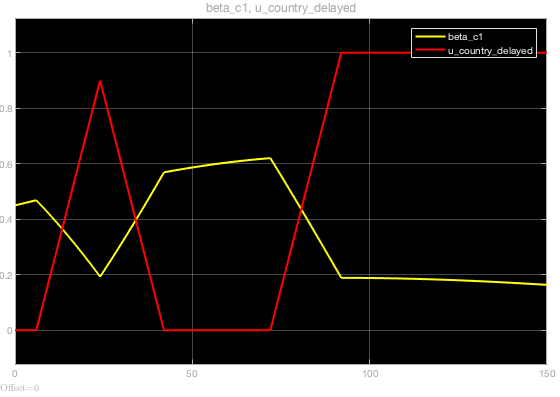
\includegraphics[width=0.75\textwidth]{Figures/hakon/A_150_mpc}
  \caption{%hakon
    Control signal $u(t)$ and resulting transmission rate $\beta_c(t)$ under MPC
    over 150~days. The 5-day transport delay is visible: the control signal activates
    early to suppress healthcare demand before it reaches the reference threshold.}
  \label{fig:mpc_A_150}
\end{figure}

There is a delay of 5~sample times between the MPC output and the resulting change in transmission due to the transport delay block.
The delayed control signal activates early in order to suppress healthcare demand and is reduced to zero between the peaks of infections and healthcare demand.
The control signal increases again as infections start to rise in the second wave scenario, and remains at its highest level for the remaining simulation time within the 150-day window.

\subsection{Long-Term MPC Behaviour (500~Days)}
\label{sec:mpc_500}

%hakon
Figure~\ref{fig:mpc_A_500} shows the long-term control signal behaviour over 500~days.
This extended simulation reveals the MPC's strategy for suppressing secondary and tertiary epidemic waves.

\begin{figure}[ht]
  \centering
  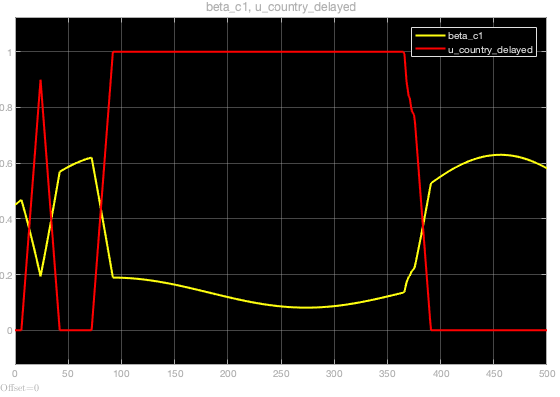
\includegraphics[width=0.75\textwidth]{Figures/hakon/A_500_mpc}
  \caption{%hakon
    Long-term control signal behaviour under MPC over 500~days.
    The MPC maintains strong intervention for approximately 300~days to suppress
    the second and third waves shown in the uncontrolled scenario.}
  \label{fig:mpc_A_500}
\end{figure}

The MPC is observed to maintain intervention for approximately 300~sample times in order to suppress the second and third waves.
This results in a prolonged period of strong control action, which may appear excessive given that the measured output falls below the reference level during this period.
However, the underlying cause is the persistent low-level infection in the normalised compartmental model: since compartment values approach zero but never exactly reach it, the controller maintains intervention to prevent future growth.

\subsection{Hospital Load Ratio}
\label{sec:hratio}

%hakon
Figure~\ref{fig:mpc_C_500} shows the hospital load ratio $H_{\mathrm{ratio}}$ under MPC control compared to the reference threshold $H_{\mathrm{ref}} = 0.8$ over 500~days.
Figure~\ref{fig:no_C_500} shows the same ratio without control.

\begin{figure}[ht]
  \centering
  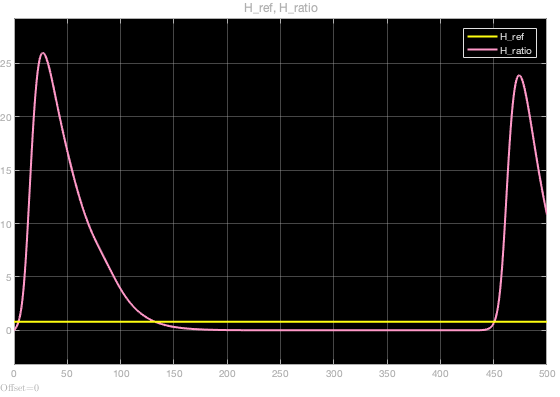
\includegraphics[width=0.75\textwidth]{Figures/hakon/C_500_mpc}
  \caption{%hakon
    Hospital load ratio $H_{\mathrm{ratio}}$ under MPC control over 500~days,
    compared to the reference threshold $H_{\mathrm{ref}} = 0.8$ (dashed line).
    The controller keeps the ratio near or below the threshold for most of the horizon.}
  \label{fig:mpc_C_500}
\end{figure}

\begin{figure}[ht]
  \centering
  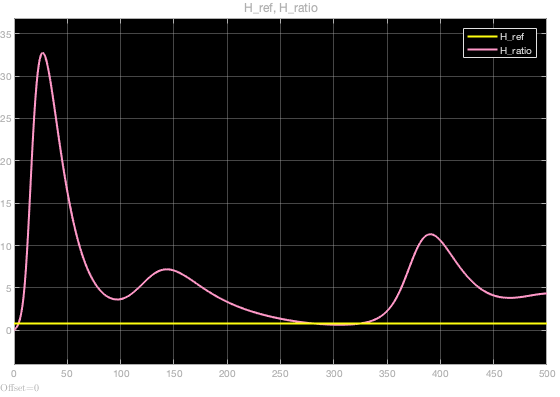
\includegraphics[width=0.75\textwidth]{Figures/hakon/C_500_no}
  \caption{%hakon
    Hospital load ratio without MPC control over 500~days.
    The healthcare system remains above capacity ($H_{\mathrm{ratio}} > 1$)
    until approximately 260~days, and is again overloaded after 65~days of recovery.}
  \label{fig:no_C_500}
\end{figure}

Without control, the healthcare system experiences significantly higher strain.
The hospital load ratio does not fall below capacity (ratio $= 1.0$) until approximately 260~sample times, and then exceeds capacity again after only a 65-day respite.
Under MPC control, the ratio is kept near or below the 0.8 reference threshold for the majority of the 500-day horizon, demonstrating effective long-term epidemic management at the macro level.
